% Created by tikzDevice version 0.12.3.1 on 2022-05-01 19:43:51
% !TEX encoding = UTF-8 Unicode
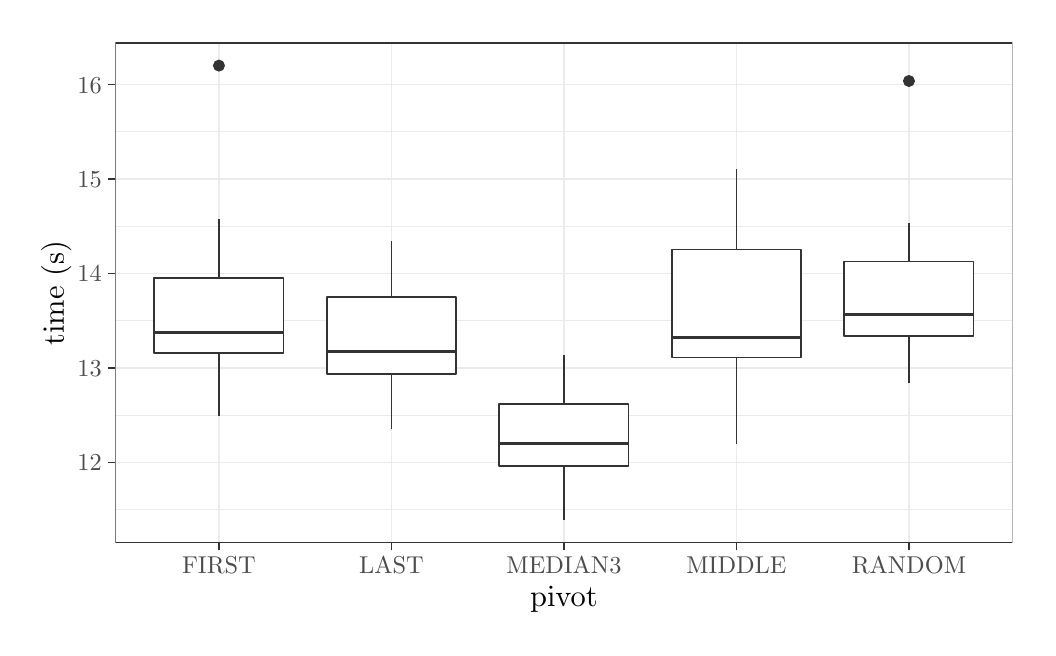
\begin{tikzpicture}[x=1pt,y=1pt]
\definecolor{fillColor}{RGB}{255,255,255}
\path[use as bounding box,fill=fillColor,fill opacity=0.00] (0,0) rectangle (361.35,216.81);
\begin{scope}
\path[clip] (  0.00,  0.00) rectangle (361.35,216.81);
\definecolor{drawColor}{RGB}{255,255,255}
\definecolor{fillColor}{RGB}{255,255,255}

\path[draw=drawColor,line width= 0.6pt,line join=round,line cap=round,fill=fillColor] (  0.00,  0.00) rectangle (361.35,216.81);
\end{scope}
\begin{scope}
\path[clip] ( 31.71, 30.69) rectangle (355.85,211.31);
\definecolor{fillColor}{RGB}{255,255,255}

\path[fill=fillColor] ( 31.71, 30.69) rectangle (355.85,211.31);
\definecolor{drawColor}{gray}{0.92}

\path[draw=drawColor,line width= 0.3pt,line join=round] ( 31.71, 42.62) --
	(355.85, 42.62);

\path[draw=drawColor,line width= 0.3pt,line join=round] ( 31.71, 76.76) --
	(355.85, 76.76);

\path[draw=drawColor,line width= 0.3pt,line join=round] ( 31.71,110.90) --
	(355.85,110.90);

\path[draw=drawColor,line width= 0.3pt,line join=round] ( 31.71,145.03) --
	(355.85,145.03);

\path[draw=drawColor,line width= 0.3pt,line join=round] ( 31.71,179.17) --
	(355.85,179.17);

\path[draw=drawColor,line width= 0.6pt,line join=round] ( 31.71, 59.69) --
	(355.85, 59.69);

\path[draw=drawColor,line width= 0.6pt,line join=round] ( 31.71, 93.83) --
	(355.85, 93.83);

\path[draw=drawColor,line width= 0.6pt,line join=round] ( 31.71,127.96) --
	(355.85,127.96);

\path[draw=drawColor,line width= 0.6pt,line join=round] ( 31.71,162.10) --
	(355.85,162.10);

\path[draw=drawColor,line width= 0.6pt,line join=round] ( 31.71,196.23) --
	(355.85,196.23);

\path[draw=drawColor,line width= 0.6pt,line join=round] ( 69.11, 30.69) --
	( 69.11,211.31);

\path[draw=drawColor,line width= 0.6pt,line join=round] (131.45, 30.69) --
	(131.45,211.31);

\path[draw=drawColor,line width= 0.6pt,line join=round] (193.78, 30.69) --
	(193.78,211.31);

\path[draw=drawColor,line width= 0.6pt,line join=round] (256.12, 30.69) --
	(256.12,211.31);

\path[draw=drawColor,line width= 0.6pt,line join=round] (318.45, 30.69) --
	(318.45,211.31);
\definecolor{drawColor}{gray}{0.20}
\definecolor{fillColor}{gray}{0.20}

\path[draw=drawColor,line width= 0.4pt,line join=round,line cap=round,fill=fillColor] ( 69.11,203.10) circle (  1.96);

\path[draw=drawColor,line width= 0.6pt,line join=round] ( 69.11,126.42) -- ( 69.11,147.56);

\path[draw=drawColor,line width= 0.6pt,line join=round] ( 69.11, 99.32) -- ( 69.11, 76.36);
\definecolor{fillColor}{RGB}{255,255,255}

\path[draw=drawColor,line width= 0.6pt,line join=round,line cap=round,fill=fillColor] ( 45.74,126.42) --
	( 45.74, 99.32) --
	( 92.49, 99.32) --
	( 92.49,126.42) --
	( 45.74,126.42) --
	cycle;

\path[draw=drawColor,line width= 1.1pt,line join=round] ( 45.74,106.79) -- ( 92.49,106.79);

\path[draw=drawColor,line width= 0.6pt,line join=round] (131.45,119.41) -- (131.45,139.70);

\path[draw=drawColor,line width= 0.6pt,line join=round] (131.45, 91.59) -- (131.45, 71.93);

\path[draw=drawColor,line width= 0.6pt,line join=round,line cap=round,fill=fillColor] (108.07,119.41) --
	(108.07, 91.59) --
	(154.82, 91.59) --
	(154.82,119.41) --
	(108.07,119.41) --
	cycle;

\path[draw=drawColor,line width= 1.1pt,line join=round] (108.07, 99.94) -- (154.82, 99.94);

\path[draw=drawColor,line width= 0.6pt,line join=round] (193.78, 80.84) -- (193.78, 98.51);

\path[draw=drawColor,line width= 0.6pt,line join=round] (193.78, 58.36) -- (193.78, 38.90);

\path[draw=drawColor,line width= 0.6pt,line join=round,line cap=round,fill=fillColor] (170.41, 80.84) --
	(170.41, 58.36) --
	(217.16, 58.36) --
	(217.16, 80.84) --
	(170.41, 80.84) --
	cycle;

\path[draw=drawColor,line width= 1.1pt,line join=round] (170.41, 66.56) -- (217.16, 66.56);

\path[draw=drawColor,line width= 0.6pt,line join=round] (256.12,136.69) -- (256.12,165.64);

\path[draw=drawColor,line width= 0.6pt,line join=round] (256.12, 97.57) -- (256.12, 66.31);

\path[draw=drawColor,line width= 0.6pt,line join=round,line cap=round,fill=fillColor] (232.74,136.69) --
	(232.74, 97.57) --
	(279.49, 97.57) --
	(279.49,136.69) --
	(232.74,136.69) --
	cycle;

\path[draw=drawColor,line width= 1.1pt,line join=round] (232.74,104.90) -- (279.49,104.90);
\definecolor{fillColor}{gray}{0.20}

\path[draw=drawColor,line width= 0.4pt,line join=round,line cap=round,fill=fillColor] (318.45,197.54) circle (  1.96);

\path[draw=drawColor,line width= 0.6pt,line join=round] (318.45,132.34) -- (318.45,146.38);

\path[draw=drawColor,line width= 0.6pt,line join=round] (318.45,105.37) -- (318.45, 88.31);
\definecolor{fillColor}{RGB}{255,255,255}

\path[draw=drawColor,line width= 0.6pt,line join=round,line cap=round,fill=fillColor] (295.07,132.34) --
	(295.07,105.37) --
	(341.82,105.37) --
	(341.82,132.34) --
	(295.07,132.34) --
	cycle;

\path[draw=drawColor,line width= 1.1pt,line join=round] (295.07,113.16) -- (341.82,113.16);

\path[draw=drawColor,line width= 0.6pt,line join=round,line cap=round] ( 31.71, 30.69) rectangle (355.85,211.31);
\end{scope}
\begin{scope}
\path[clip] (  0.00,  0.00) rectangle (361.35,216.81);
\definecolor{drawColor}{gray}{0.30}

\node[text=drawColor,anchor=base east,inner sep=0pt, outer sep=0pt, scale=  0.88] at ( 26.76, 56.66) {12};

\node[text=drawColor,anchor=base east,inner sep=0pt, outer sep=0pt, scale=  0.88] at ( 26.76, 90.80) {13};

\node[text=drawColor,anchor=base east,inner sep=0pt, outer sep=0pt, scale=  0.88] at ( 26.76,124.93) {14};

\node[text=drawColor,anchor=base east,inner sep=0pt, outer sep=0pt, scale=  0.88] at ( 26.76,159.07) {15};

\node[text=drawColor,anchor=base east,inner sep=0pt, outer sep=0pt, scale=  0.88] at ( 26.76,193.20) {16};
\end{scope}
\begin{scope}
\path[clip] (  0.00,  0.00) rectangle (361.35,216.81);
\definecolor{drawColor}{gray}{0.20}

\path[draw=drawColor,line width= 0.6pt,line join=round] ( 28.96, 59.69) --
	( 31.71, 59.69);

\path[draw=drawColor,line width= 0.6pt,line join=round] ( 28.96, 93.83) --
	( 31.71, 93.83);

\path[draw=drawColor,line width= 0.6pt,line join=round] ( 28.96,127.96) --
	( 31.71,127.96);

\path[draw=drawColor,line width= 0.6pt,line join=round] ( 28.96,162.10) --
	( 31.71,162.10);

\path[draw=drawColor,line width= 0.6pt,line join=round] ( 28.96,196.23) --
	( 31.71,196.23);
\end{scope}
\begin{scope}
\path[clip] (  0.00,  0.00) rectangle (361.35,216.81);
\definecolor{drawColor}{gray}{0.20}

\path[draw=drawColor,line width= 0.6pt,line join=round] ( 69.11, 27.94) --
	( 69.11, 30.69);

\path[draw=drawColor,line width= 0.6pt,line join=round] (131.45, 27.94) --
	(131.45, 30.69);

\path[draw=drawColor,line width= 0.6pt,line join=round] (193.78, 27.94) --
	(193.78, 30.69);

\path[draw=drawColor,line width= 0.6pt,line join=round] (256.12, 27.94) --
	(256.12, 30.69);

\path[draw=drawColor,line width= 0.6pt,line join=round] (318.45, 27.94) --
	(318.45, 30.69);
\end{scope}
\begin{scope}
\path[clip] (  0.00,  0.00) rectangle (361.35,216.81);
\definecolor{drawColor}{gray}{0.30}

\node[text=drawColor,anchor=base,inner sep=0pt, outer sep=0pt, scale=  0.88] at ( 69.11, 19.68) {FIRST};

\node[text=drawColor,anchor=base,inner sep=0pt, outer sep=0pt, scale=  0.88] at (131.45, 19.68) {LAST};

\node[text=drawColor,anchor=base,inner sep=0pt, outer sep=0pt, scale=  0.88] at (193.78, 19.68) {MEDIAN3};

\node[text=drawColor,anchor=base,inner sep=0pt, outer sep=0pt, scale=  0.88] at (256.12, 19.68) {MIDDLE};

\node[text=drawColor,anchor=base,inner sep=0pt, outer sep=0pt, scale=  0.88] at (318.45, 19.68) {RANDOM};
\end{scope}
\begin{scope}
\path[clip] (  0.00,  0.00) rectangle (361.35,216.81);
\definecolor{drawColor}{RGB}{0,0,0}

\node[text=drawColor,anchor=base,inner sep=0pt, outer sep=0pt, scale=  1.10] at (193.78,  7.64) {pivot};
\end{scope}
\begin{scope}
\path[clip] (  0.00,  0.00) rectangle (361.35,216.81);
\definecolor{drawColor}{RGB}{0,0,0}

\node[text=drawColor,rotate= 90.00,anchor=base,inner sep=0pt, outer sep=0pt, scale=  1.10] at ( 13.08,121.00) {time (s)};
\end{scope}
\end{tikzpicture}
